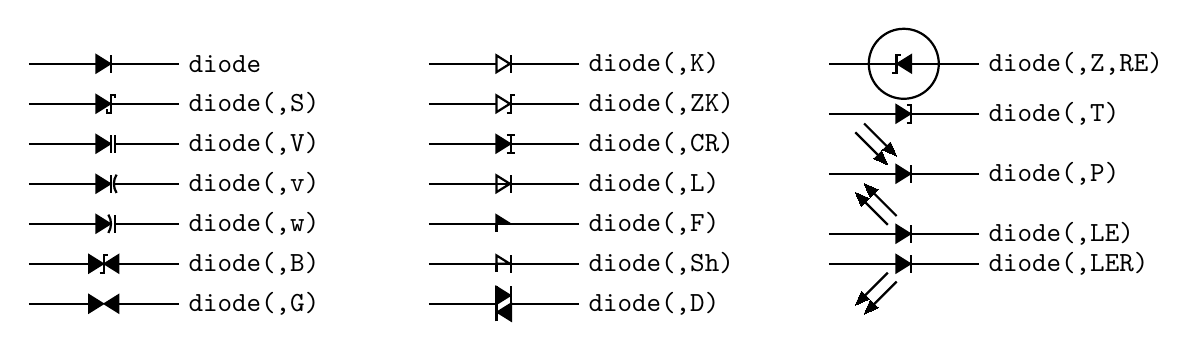
\begin{tikzpicture}[scale=2.54]
% dpic version 2020.03.01 option -g for TikZ and PGF 1.01
\ifx\dpiclw\undefined\newdimen\dpiclw\fi
\global\def\dpicdraw{\draw[line width=\dpiclw]}
\global\def\dpicstop{;}
\dpiclw=0.8bp
\dpiclw=0.8bp
\dpicdraw (0,0)
 --(0.338916,0)\dpicstop
\global\let\dpicshdraw=\dpicdraw\global\def\dpicdraw{}
\global\def\dpicstop{--}
\dpicshdraw[fill=white!0!black]
\dpicdraw (0.338916,0)
 --(0.338916,0.041667)
 --(0.40555,0)
 --(0.338916,-0.041667)
 --(0.338916,0)\dpicstop
cycle; \global\let\dpicdraw=\dpicshdraw\global\def\dpicstop{;}
\dpicdraw (0.411084,-0.045718)
 --(0.411084,0.045718)\dpicstop
\dpicdraw (0.411084,0)
 --(0.75,0)\dpicstop
\draw (0.777674,0) node[right=-2bp]{{\tt diode}};
\dpicdraw (0,-0.2)
 --(0.338916,-0.2)\dpicstop
\global\let\dpicshdraw=\dpicdraw\global\def\dpicdraw{}
\global\def\dpicstop{--}
\dpicshdraw[fill=white!0!black]
\dpicdraw (0.338916,-0.2)
 --(0.338916,-0.158333)
 --(0.40555,-0.2)
 --(0.338916,-0.241667)
 --(0.338916,-0.2)\dpicstop
cycle; \global\let\dpicdraw=\dpicshdraw\global\def\dpicstop{;}
\dpicdraw (0.390251,-0.227778)
 --(0.390251,-0.245718)
 --(0.411084,-0.245718)
 --(0.411084,-0.154282)
 --(0.431918,-0.154282)
 --(0.431918,-0.172222)\dpicstop
\dpicdraw (0.411084,-0.2)
 --(0.75,-0.2)\dpicstop
\draw (0.777674,-0.2) node[right=-2bp]{{\tt diode(,S)}};
\dpicdraw (0,-0.4)
 --(0.338916,-0.4)\dpicstop
\global\let\dpicshdraw=\dpicdraw\global\def\dpicdraw{}
\global\def\dpicstop{--}
\dpicshdraw[fill=white!0!black]
\dpicdraw (0.338916,-0.4)
 --(0.338916,-0.358333)
 --(0.40555,-0.4)
 --(0.338916,-0.441667)
 --(0.338916,-0.4)\dpicstop
cycle; \global\let\dpicdraw=\dpicshdraw\global\def\dpicstop{;}
\dpicdraw (0.411084,-0.445718)
 --(0.411084,-0.354282)\dpicstop
\dpicdraw (0.431918,-0.445718)
 --(0.431918,-0.354282)\dpicstop
\dpicdraw (0.431918,-0.4)
 --(0.75,-0.4)\dpicstop
\draw (0.777674,-0.4) node[right=-2bp]{{\tt diode(,V)}};
\dpicdraw (0,-0.6)
 --(0.338916,-0.6)\dpicstop
\global\let\dpicshdraw=\dpicdraw\global\def\dpicdraw{}
\global\def\dpicstop{--}
\dpicshdraw[fill=white!0!black]
\dpicdraw (0.338916,-0.6)
 --(0.338916,-0.558333)
 --(0.40555,-0.6)
 --(0.338916,-0.641667)
 --(0.338916,-0.6)\dpicstop
cycle; \global\let\dpicdraw=\dpicshdraw\global\def\dpicstop{;}
\dpicdraw (0.411084,-0.645718)
 --(0.411084,-0.554282)\dpicstop
\dpicdraw (0.438862,-0.645718)
 ..controls (0.421179,-0.617804) and (0.421179,-0.582196)
 ..(0.438862,-0.554282)\dpicstop
\dpicdraw (0.4256,-0.6)
 --(0.431918,-0.6)\dpicstop
\dpicdraw (0.431918,-0.6)
 --(0.75,-0.6)\dpicstop
\draw (0.777674,-0.6) node[right=-2bp]{{\tt diode(,v)}};
\dpicdraw (0,-0.8)
 --(0.338916,-0.8)\dpicstop
\global\let\dpicshdraw=\dpicdraw\global\def\dpicdraw{}
\global\def\dpicstop{--}
\dpicshdraw[fill=white!0!black]
\dpicdraw (0.338916,-0.8)
 --(0.338916,-0.758333)
 --(0.40555,-0.8)
 --(0.338916,-0.841667)
 --(0.338916,-0.8)\dpicstop
cycle; \global\let\dpicdraw=\dpicshdraw\global\def\dpicstop{;}
\dpicdraw (0.397822,-0.754282)
 ..controls (0.415505,-0.782196) and (0.415505,-0.817804)
 ..(0.397822,-0.845718)\dpicstop
\dpicdraw (0.431918,-0.845718)
 --(0.431918,-0.754282)\dpicstop
\dpicdraw (0.431918,-0.8)
 --(0.75,-0.8)\dpicstop
\draw (0.777674,-0.8) node[right=-2bp]{{\tt diode(,w)}};
\dpicdraw (0,-1)
 --(0.302831,-1)\dpicstop
\global\let\dpicshdraw=\dpicdraw\global\def\dpicdraw{}
\global\def\dpicstop{--}
\dpicshdraw[fill=white!0!black]
\dpicdraw (0.302831,-1)
 --(0.302831,-0.958333)
 --(0.369465,-1)
 --(0.302831,-1.041667)
 --(0.302831,-1)\dpicstop
cycle; \global\let\dpicdraw=\dpicshdraw\global\def\dpicstop{;}
\dpicdraw (0.354167,-1.045718)
 --(0.375,-1.045718)
 --(0.375,-0.954282)
 --(0.395833,-0.954282)\dpicstop
\global\let\dpicshdraw=\dpicdraw\global\def\dpicdraw{}
\global\def\dpicstop{--}
\dpicshdraw[fill=white!0!black]
\dpicdraw (0.447169,-1)
 --(0.447169,-0.958333)
 --(0.380535,-1)
 --(0.447169,-1.041667)
 --(0.447169,-1)\dpicstop
cycle; \global\let\dpicdraw=\dpicshdraw\global\def\dpicstop{;}
\dpicdraw (0.447169,-1)
 --(0.75,-1)\dpicstop
\draw (0.777674,-1) node[right=-2bp]{{\tt diode(,B)}};
\dpicdraw (0,-1.2)
 --(0.302831,-1.2)\dpicstop
\global\let\dpicshdraw=\dpicdraw\global\def\dpicdraw{}
\global\def\dpicstop{--}
\dpicshdraw[fill=white!0!black]
\dpicdraw (0.302831,-1.2)
 --(0.302831,-1.158333)
 --(0.369465,-1.2)
 --(0.302831,-1.241667)
 --(0.302831,-1.2)\dpicstop
cycle; \global\let\dpicdraw=\dpicshdraw\global\def\dpicstop{;}
\global\let\dpicshdraw=\dpicdraw\global\def\dpicdraw{}
\global\def\dpicstop{--}
\dpicshdraw[fill=white!0!black]
\dpicdraw (0.447169,-1.2)
 --(0.447169,-1.158333)
 --(0.380535,-1.2)
 --(0.447169,-1.241667)
 --(0.447169,-1.2)\dpicstop
cycle; \global\let\dpicdraw=\dpicshdraw\global\def\dpicstop{;}
\dpicdraw (0.447169,-1.2)
 --(0.75,-1.2)\dpicstop
\draw (0.777674,-1.2) node[right=-2bp]{{\tt diode(,G)}};
\dpicdraw (2,0)
 --(2.338916,0)\dpicstop
\dpicdraw (2.338916,0)
 --(2.338916,0.041667)
 --(2.40555,0)
 --(2.338916,-0.041667)
 --(2.338916,0)\dpicstop
\dpicdraw (2.411084,-0.045718)
 --(2.411084,0.045718)\dpicstop
\dpicdraw (2.411084,0)
 --(2.75,0)\dpicstop
\draw (2.777674,0) node[right=-2bp]{{\tt diode(,K)}};
\dpicdraw (2,-0.2)
 --(2.338916,-0.2)\dpicstop
\dpicdraw (2.338916,-0.2)
 --(2.338916,-0.158333)
 --(2.40555,-0.2)
 --(2.338916,-0.241667)
 --(2.338916,-0.2)\dpicstop
\dpicdraw (2.390251,-0.245718)
 --(2.411084,-0.245718)
 --(2.411084,-0.154282)
 --(2.431918,-0.154282)\dpicstop
\dpicdraw (2.411084,-0.2)
 --(2.75,-0.2)\dpicstop
\draw (2.777674,-0.2) node[right=-2bp]{{\tt diode(,ZK)}};
\dpicdraw (2,-0.4)
 --(2.338916,-0.4)\dpicstop
\global\let\dpicshdraw=\dpicdraw\global\def\dpicdraw{}
\global\def\dpicstop{--}
\dpicshdraw[fill=white!0!black]
\dpicdraw (2.338916,-0.4)
 --(2.338916,-0.358333)
 --(2.40555,-0.4)
 --(2.338916,-0.441667)
 --(2.338916,-0.4)\dpicstop
cycle; \global\let\dpicdraw=\dpicshdraw\global\def\dpicstop{;}
\dpicdraw (2.411084,-0.445718)
 --(2.411084,-0.354282)\dpicstop
\dpicdraw (2.390251,-0.445718)
 --(2.431918,-0.445718)\dpicstop
\dpicdraw (2.390251,-0.354282)
 --(2.431918,-0.354282)\dpicstop
\dpicdraw (2.411084,-0.4)
 --(2.75,-0.4)\dpicstop
\draw (2.777674,-0.4) node[right=-2bp]{{\tt diode(,CR)}};
\dpicdraw (2,-0.6)
 --(2.338916,-0.6)\dpicstop
\dpicdraw (2.338916,-0.6)
 --(2.338916,-0.558333)
 --(2.40555,-0.6)
 --(2.338916,-0.641667)
 --(2.338916,-0.6)\dpicstop
\dpicdraw (2.338916,-0.6)
 --(2.411084,-0.6)\dpicstop
\dpicdraw (2.411084,-0.645718)
 --(2.411084,-0.554282)\dpicstop
\dpicdraw (2.411084,-0.6)
 --(2.75,-0.6)\dpicstop
\draw (2.777674,-0.6) node[right=-2bp]{{\tt diode(,L)}};
\dpicdraw (2,-0.8)
 --(2.338916,-0.8)\dpicstop
\global\let\dpicshdraw=\dpicdraw\global\def\dpicdraw{}
\global\def\dpicstop{--}
\dpicshdraw[fill=white!0!black]
\dpicdraw (2.338916,-0.8)
 --(2.338916,-0.758333)
 --(2.40555,-0.8)
 --(2.338916,-0.8)\dpicstop
cycle; \global\let\dpicdraw=\dpicshdraw\global\def\dpicstop{;}
\dpicdraw (2.338916,-0.8)
 --(2.338916,-0.841667)\dpicstop
\dpicdraw (2.411084,-0.8)
 --(2.75,-0.8)\dpicstop
\draw (2.777674,-0.8) node[right=-2bp]{{\tt diode(,F)}};
\dpicdraw (2,-1)
 --(2.338916,-1)\dpicstop
\dpicdraw (2.338916,-1)
 --(2.338916,-0.958333)
 --(2.40555,-1)
 --(2.338916,-1)\dpicstop
\dpicdraw (2.338916,-1)
 --(2.338916,-1.041667)\dpicstop
\dpicdraw (2.411084,-1.045718)
 --(2.411084,-0.954282)\dpicstop
\dpicdraw (2.411084,-1)
 --(2.75,-1)\dpicstop
\draw (2.777674,-1) node[right=-2bp]{{\tt diode(,Sh)}};
\dpicdraw (2,-1.2)
 --(2.338916,-1.2)\dpicstop
\global\let\dpicshdraw=\dpicdraw\global\def\dpicdraw{}
\global\def\dpicstop{--}
\dpicshdraw[fill=white!0!black]
\dpicdraw (2.338916,-1.158333)
 --(2.338916,-1.116667)
 --(2.40555,-1.158333)
 --(2.338916,-1.2)
 --(2.338916,-1.158333)\dpicstop
cycle; \global\let\dpicdraw=\dpicshdraw\global\def\dpicstop{;}
\dpicdraw (2.411084,-1.287385)
 --(2.411084,-1.112615)\dpicstop
\dpicdraw (2.338916,-1.287385)
 --(2.338916,-1.112615)\dpicstop
\global\let\dpicshdraw=\dpicdraw\global\def\dpicdraw{}
\global\def\dpicstop{--}
\dpicshdraw[fill=white!0!black]
\dpicdraw (2.411084,-1.241667)
 --(2.411084,-1.2)
 --(2.34445,-1.241667)
 --(2.411084,-1.283333)
 --(2.411084,-1.241667)\dpicstop
cycle; \global\let\dpicdraw=\dpicshdraw\global\def\dpicstop{;}
\dpicdraw (2.411084,-1.2)
 --(2.75,-1.2)\dpicstop
\draw (2.777674,-1.2) node[right=-2bp]{{\tt diode(,D)}};
\dpicdraw (4.75,0)
 --(4.411084,0)\dpicstop
\global\let\dpicshdraw=\dpicdraw\global\def\dpicdraw{}
\global\def\dpicstop{--}
\dpicshdraw[fill=white!0!black]
\dpicdraw (4.411084,0)
 --(4.411084,-0.041667)
 --(4.34445,0)
 --(4.411084,0.041667)
 --(4.411084,0)\dpicstop
cycle; \global\let\dpicdraw=\dpicshdraw\global\def\dpicstop{;}
\dpicdraw (4.359749,0.045718)
 --(4.338916,0.045718)
 --(4.338916,-0.045718)
 --(4.318082,-0.045718)\dpicstop
\dpicdraw (4.338916,0)
 --(4,0)\dpicstop
\dpicdraw (4.375,0) circle (0.068898in)\dpicstop
\draw (4.777674,0) node[right=-2bp]{{\tt diode(,Z,RE)}};
\dpicdraw (4,-0.25)
 --(4.338916,-0.25)\dpicstop
\global\let\dpicshdraw=\dpicdraw\global\def\dpicdraw{}
\global\def\dpicstop{--}
\dpicshdraw[fill=white!0!black]
\dpicdraw (4.338916,-0.25)
 --(4.338916,-0.208333)
 --(4.40555,-0.25)
 --(4.338916,-0.291667)
 --(4.338916,-0.25)\dpicstop
cycle; \global\let\dpicdraw=\dpicshdraw\global\def\dpicstop{;}
\dpicdraw (4.390251,-0.295718)
 --(4.411084,-0.295718)
 --(4.411084,-0.204282)
 --(4.390251,-0.204282)\dpicstop
\dpicdraw (4.411084,-0.25)
 --(4.75,-0.25)\dpicstop
\draw (4.777674,-0.25) node[right=-2bp]{{\tt diode(,T)}};
\dpicdraw (4,-0.55)
 --(4.338916,-0.55)\dpicstop
\filldraw[line width=0bp](4.269213,-0.43037)
 --(4.339362,-0.461236)
 --(4.308496,-0.391087) --cycle\dpicstop
\dpicdraw (4.176728,-0.298602)
 --(4.328524,-0.450398)\dpicstop
\filldraw[line width=0bp](4.225018,-0.474565)
 --(4.295168,-0.50543)
 --(4.264302,-0.435281) --cycle\dpicstop
\dpicdraw (4.132533,-0.342796)
 --(4.284329,-0.494592)\dpicstop
\global\let\dpicshdraw=\dpicdraw\global\def\dpicdraw{}
\global\def\dpicstop{--}
\dpicshdraw[fill=white!0!black]
\dpicdraw (4.338916,-0.55)
 --(4.338916,-0.508333)
 --(4.40555,-0.55)
 --(4.338916,-0.591667)
 --(4.338916,-0.55)\dpicstop
cycle; \global\let\dpicdraw=\dpicshdraw\global\def\dpicstop{;}
\dpicdraw (4.411084,-0.595718)
 --(4.411084,-0.504282)\dpicstop
\dpicdraw (4.411084,-0.55)
 --(4.75,-0.55)\dpicstop
\draw (4.777674,-0.55) node[right=-2bp]{{\tt diode(,P)}};
\dpicdraw (4,-0.85)
 --(4.338916,-0.85)\dpicstop
\filldraw[line width=0bp](4.202683,-0.673662)
 --(4.132533,-0.642796)
 --(4.163399,-0.712945) --cycle\dpicstop
\dpicdraw (4.295168,-0.80543)
 --(4.143372,-0.653634)\dpicstop
\filldraw[line width=0bp](4.246877,-0.629467)
 --(4.176728,-0.598602)
 --(4.207593,-0.668751) --cycle\dpicstop
\dpicdraw (4.339362,-0.761236)
 --(4.187566,-0.60944)\dpicstop
\global\let\dpicshdraw=\dpicdraw\global\def\dpicdraw{}
\global\def\dpicstop{--}
\dpicshdraw[fill=white!0!black]
\dpicdraw (4.338916,-0.85)
 --(4.338916,-0.808333)
 --(4.40555,-0.85)
 --(4.338916,-0.891667)
 --(4.338916,-0.85)\dpicstop
cycle; \global\let\dpicdraw=\dpicshdraw\global\def\dpicstop{;}
\dpicdraw (4.411084,-0.895718)
 --(4.411084,-0.804282)\dpicstop
\dpicdraw (4.411084,-0.85)
 --(4.75,-0.85)\dpicstop
\draw (4.777674,-0.85) node[right=-2bp]{{\tt diode(,LE)}};
\dpicdraw (4,-1)
 --(4.338916,-1)\dpicstop
\filldraw[line width=0bp](4.207593,-1.181249)
 --(4.176728,-1.251398)
 --(4.246877,-1.220533) --cycle\dpicstop
\dpicdraw (4.339362,-1.088764)
 --(4.187566,-1.24056)\dpicstop
\filldraw[line width=0bp](4.163399,-1.137055)
 --(4.132533,-1.207204)
 --(4.202683,-1.176338) --cycle\dpicstop
\dpicdraw (4.295168,-1.04457)
 --(4.143372,-1.196366)\dpicstop
\global\let\dpicshdraw=\dpicdraw\global\def\dpicdraw{}
\global\def\dpicstop{--}
\dpicshdraw[fill=white!0!black]
\dpicdraw (4.338916,-1)
 --(4.338916,-0.958333)
 --(4.40555,-1)
 --(4.338916,-1.041667)
 --(4.338916,-1)\dpicstop
cycle; \global\let\dpicdraw=\dpicshdraw\global\def\dpicstop{;}
\dpicdraw (4.411084,-1.045718)
 --(4.411084,-0.954282)\dpicstop
\dpicdraw (4.411084,-1)
 --(4.75,-1)\dpicstop
\draw (4.777674,-1) node[right=-2bp]{{\tt diode(,LER)}};
\end{tikzpicture}
\vspace*{-0.5\baselineskip}
